% Quick start guide
\documentclass[table, dvipsnames]{beamer}

\usetheme{Hannover}
\usefonttheme[onlymath]{serif}
\usecolortheme{rose}
\usepackage{mathpazo}
\usepackage{multirow}

\title{Restricted parking functions}
\author{Alan Kappler, Jayden Thadani}
\date{29th May 2024}

\begin{document}

\setbeamertemplate{sidebar left}[sidebar theme]


\begin{frame}
    \titlepage
\end{frame}

\begin{frame}{We will talk about}
    \tableofcontents
\end{frame}

\section{What restricted parking functions are}

\begin{frame}{What is a parking function?}
	\only<1, 2, 3, 4>{
		Imagine a parking spots on a one-way street, with $s$ spots to park in. $c = s$ cars, labelled $1$ to $s$, wish to park in the lot, entering the street one at a time. \pause \\~
	
		They each prefer a particular spot. This can be thought of as a \textit{preference function} $\pi: [s] \to [s]$ or a \textit{preference list} $\pi \in [s]^{s}$ that maps each car to their preference. \pause \\~
	
		Each car first goes to their preferred spot and parks there if they can. If the spot is full, then they continue along the street until they find an empty spot. If they don't find an empty spot, they don't park. \pause \\~
	
		If all cars park successfully, $\pi$ is a \textit{parking function}.
	}
	\only<5>{
		We can characterise whether a preference list is a parking function just by its \textit{non-decreasing} rearrangement.
		\begin{theorem}[the Catalan condition for parking functions]
			A preference list $\pi \in [s]^{s}$ is a parking function if and only if, its non-decreasing rearrangement $\pi' = (\pi'_{1}, \dots, \pi_{s}')$ gives $\pi'_{i} \le i$ for all $i \in [s]$.
		\end{theorem}
		That is, $\pi$ is a parking function when at least $i$ cars want to park in the first $i$ slots for all $i$. \\~ 

		This means parking functions are permutation invariant! 
	}
	\only<6>{
		\begin{example}[parking functions]
			$(1, 2, 2, 2)$, $(2, 1, 2, 2)$, $(2, 2, 1, 2)$ and $(2, 2, 2, 1)$ are all parking functions of length $4$ --- the cars preferring spot $2$ fill up spots $2, 3, 4$ in order and the remaining car parks in spot $1$.
		\end{example}
		\begin{example}[non-parking functions]
			$(1, 3, 3, 3)$ and its permutations are not parking functions --- three cars are trying to park in spots $3$ and $4$.
		\end{example}
	}
\end{frame}

\begin{frame}{What is a restricted parking function?}
	\only<1, 2, 3>{
		Imagine now that we have more cars (say $c > s$ of them) than spots. Some cars will be unable to park. How can we minimise this \textit{defect}? \pause \\~
		
		The minimum defect preference lists are exactly the parking function of length $c$, where the cars' preferences are restricted to $[s]$. Just forget about the last $c - s$ slots! \pause \\~
		
		% Clearly if we have a parking function $\pi : [c] \to [c]$, then there will be $s$ cars parked in the first $s$ slots. If we have a preference list $\pi : [c] \to [s]$, then after the first $s$ slots are filled, the remaining cars will park in order in the last $c - s$ slots, forming a parking function.
		This motivates thinking about parking functions on $[c]$ with preferences restricted to some subset $[s] \subset [c]$. More generally, we can interpret parking functions restricted to \textit{any} subset $S \subset [c]$. \\

	}
	\only<4>{
		\begin{example}[many cars in one spot]
			Restricting our $c$ cars to prefer a certain spots $s \in S$ such that $s = 1 \pmod g$ for some gap $g$, corresponds to allowing multiple cars to park in one spot. \\~

			Just think of the $g$ spots between any two consecutive $s_{1}, s_{2} \in S$ as forming one parking spot at $s$ able to hold $g$ cars.
		\end{example} ~

		Thus, we define
		\begin{definition}[restricted parking function]
			A restricted parking function of $c$ cars on $S\subset [c]$ is a parking function $\pi : [c] \to [c]$ such that $\operatorname{range} \pi \subseteq S.$
		\end{definition}
			}
\end{frame}

\section{How to count parking functions}

\begin{frame}{Counting parking functions}
	\only<1, 2>{
			Pollack came up with a neat \textit{circular argument} to enumerate parking functions. \\~ \pause

			Consider $n+1$ parking spots in a circle and $n$ cars allowed to prefer any of the spots:\\~

			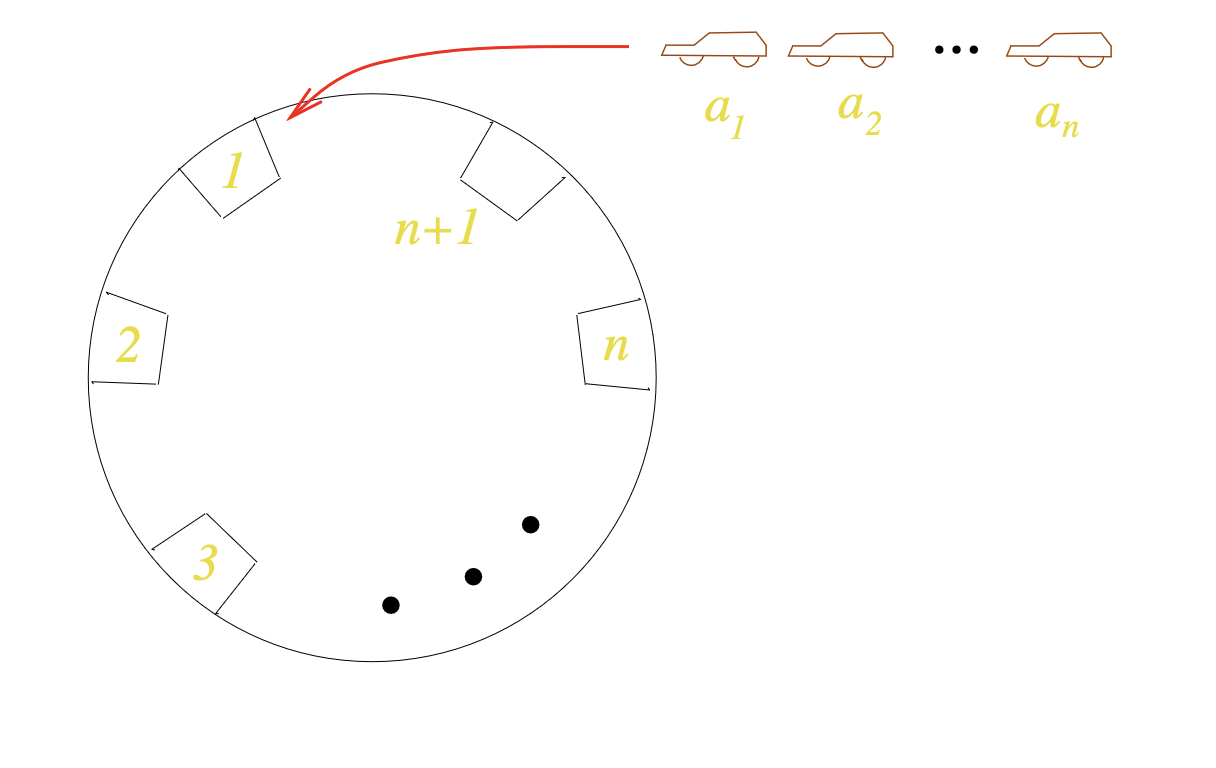
\includegraphics[scale=0.35]{circle-parking.png}
	}
    \only<3>{
	    	Ultimately all spots are filled but one. Thus, each of the $(n + 1)^{n}$ preference lists here corresponds to a parking function on $n$ cars on the $n$ filled spots. \\~
		
		Each parking function is represented $n+1$ times in the circle. Thus, there are
    		\[
    			P_{n} = \frac{(n+1)^n}{n+1} = (n+1)^{n-1}
    		\]
    		total parking functions on $n$ cars. \pause \\~

		This argument will be important later!
	}
\end{frame}

\section{How to count restrictions to $[s] \subset [c]$}

\begin{frame}
	\frametitle{The easiest case --- $S = [c - 1]$}
		These preference lists are exactly the parking functions of length $c$ where no one wants to park in the $c$th spot. \\~

		We can subtract the ``bad" parking functions --- \pause
		\begin{enumerate}
			\item choose the car that wants to park in spot $c$ in one of $c$ ways \pause
			\item the rest of the preference list must be one of $(s + 1)^{s - 1}$ parking functions of length $s = c - 1$. \pause
	\end{enumerate}~
	
	There are $P_{c} - \binom{c}{1} P_{c - 1}$ parking preference lists left. \pause \\~

	Does this generalise?
\end{frame}	

\begin{frame}{Counting restricted parking functions for $S = [s]$}
    \begin{theorem}
        The number of restricted parking functions of $c$ cars on $[s]\subseteq [c]$ may be expressed as
        \[s^c-\sum_{i=1}^s \binom{c}{i-1}i^{i-2}(s-i)^{c-i+1}\]
        or as
        \[\sum_{i=s}^{c} (-1)^{c - i} \binom{c}{i}(i+1)^{i-1}(i - s + 1)^{c-i}.\]
    \end{theorem}	
\end{frame}

\begin{frame}
\begin{proof}[Proof (claim 1)]
    Instead of counting directly, we count the number of preference functions with image within $[s]$ which are \textit{not} parking functions. We may then subtract this from $s^c$.\\~\pause
    
    Consider some restricted non-parking function. Since at least one car did not park, there is at least one empty spot; call the first such empty spot $i.$ How many non-parking functions are there that yield a given spot $i$?\\~\pause

    The $i-1$ spots prior to spot $i$ must have $i-1$ cars in them. There are $\binom{c}{i-1}$ ways to choose these cars, $i^{i-2}$ ways to assemble them in the first $i-1$ spots, and $(n-i)^{c-i+1}$ ways to choose spots for the rest.\\~\pause

    Summing over all $i$ gives the desired total of $s^c-\sum_{i=1}^s \binom{c}{i-1}i^{i-2}(s-i)^{c-i+1}.$
\end{proof}
\end{frame}

\begin{frame}
\begin{proof}[Proof (claim 2)]
We count parking functions with cars painted (say) indigo and red, such that the $i\ge s$ indigo cars form a parking function on the first $i$ slots, and the remaining $c-i$ red cars all prefer spots from $s+1$ to $i+1.$ We count these with a factor of $(-1)^{c-i},$ $c-i$ the number of red cars.\\~\pause

We next define an \textit{involution} on this set: in a given parking function, $x$ be the first car such that no other car prefers a later spot. Our involution repaints $x$: red if it's indigo, indigo if it's red.\\~\pause

This gives us a correspondence between functions counted positively and negatively, so everything cancels out with one \textit{exception}: restricted parking functions with everything indigo. This is precisely what we're trying to count.
\end{proof}
\end{frame}

\begin{frame}
    These two proofs together show that \begin{align*}s^c-&\sum_{i=1}^s \binom{c}{i-1}i^{i-2}(n-i)^{c-i+1}\\=&\sum_{i=s}^{c} (-1)^{c - i} \binom{c}{i}(i+1)^{i-1}(i - s + 1)^{c-i}.\end{align*} Some rearrangement and relabeling gives us the formula $$s^c=\sum_{i=0}^c \binom{c}{i}(i+1)^{i-1}(s-i-1)^{c-i}.$$ This is a special case of an identity called \textit{Abel's binomial theorem}: which has no standard combinatorial proof, as far as we can tell.
\end{frame}

\section{A strange coincidence}

\begin{frame}
	\only<1>{
	\frametitle{A strange coincidence ...}
	From our formulas, we can get this table ---
	\begin{block}{\# preference lists such that $c - s$ cars can't park}
		\begin{center}
			\begin{tabular}{c || r | r r r r r r}
				& \multicolumn{7}{c}{$c$ cars} \\ \hline \hline
				\multirow{7}{*}{\rotatebox[origin=c]{90}{prefer first $s$ spots}}  & & $1$ & $2$ & $3$ & $4$ & $5$ & $6$ \\ \cline{2 - 8}
												       & $1$ & $1$ & $1$ & $1$ & $1$ & $1$ & $1$ \\
												       & $2$ & & $3$  &  $7$ & $15$ & $31$ & $63$ \\
												       & $3$ & & & $16$ & $61$ & $206$ & $659$ \\ 
												       & $4$ & & & & $125$ & $671$ & $3130$ \\
												       & $5$ & & & & &  $1296$ & $9031$ \\
												       & $6$ & & & & & & $144995$
			\end{tabular}
		\end{center}
	\end{block}
	}
	\only<2>{
	\frametitle{... hyperplane arrangements!}
	Which the OEIS tells us are the number of regions in the {\color{blue} $c$-Linial}, {\color{red} $C_{c}$-Shi}, and {\color{ForestGreen} $K_{c}$-Shi} hyperplane arrangements.
	\begin{block}{\# preference lists such that $c - s$ cars can't park}
		\begin{center}
			\begin{tabular}{c || r | r r r r r r}
				& \multicolumn{7}{c}{$c$ cars} \\ \hline \hline
				\multirow{7}{*}{\rotatebox[origin=c]{90}{prefer first $s$ spots}}  & & $1$ & $2$ & $3$ & $4$ & $5$ & $6$ \\ \cline{2 - 8}
												       & $1$ & $1$ & $1$ & $1$ & $1$ & $1$ & $1$ \\
												       & $2$ & & \color{blue} $3$ & \color{blue} $7$ & \color{blue} $15$ & \color{blue} $31$ & \color{blue} $63$ \\
												       & $3$ & & & \color{red} \color{red} $16$ & \color{red} $61$ & \color{red} $206$ & \color{red} $659$ \\ 
												       & $4$ & & & & \color{ForestGreen} $125$ & $671$ & $3130$ \\
												       & $5$ & & & & & \color{ForestGreen} $1296$ & $9031$ \\
												       & $6$ & & & & & & \color{ForestGreen} $144995$
			\end{tabular}
		\end{center}
	\end{block}
	}

\end{frame}

\section{Modular restrictions}

\begin{frame}{Modular restrictions}
    \begin{theorem}
        Let $S$ be the set of elements in $[gs-1]$ equal to 1 mod $g$; then the number of restricted parking functions of $gs-1$ cars on $S$ is $s^{gs-2}.$
    \end{theorem}\pause
    \begin{proof}
        We use a circle argument similar to Pollak's. Consider $s$ spots in a circle, each of which holds $g$ cars, and let $gs-1$ cars enter; there are $s^{gs-1}$ possible preference lists. Each leads to a parking function in which one spot has $s-1$ cars; this break can happen in $s$ places. Thus the total number of parking functions is $\frac{s^{gs-1}}{s}=s^{gs-2}.$
    \end{proof}
\end{frame}

\begin{frame}{Harder versions}
    Further results on modular restrictions are significantly harder to come by, with more and more nested sums as you retreat further from $gs-1.$ Case in point:\pause\\~

    \begin{theorem}
        Let $S$ be the set of elements in $[gs-2]$ equal to 1 mod $g$; then the number of restricted parking functions of $gs-2$ cars on $S$ is $$s^{gs-3}-\frac{1}{2}\sum_{i=1}^{n-1}\binom{gs-2}{gi-1}i^{gi-2}(s-i)^{g(s-i)-2}.$$
    \end{theorem}    
\end{frame}



\end{document}
